\documentclass[11pt]{article}

\usepackage[a4paper,margin=0.88in]{geometry}
\usepackage{amsmath,amssymb,amsthm}
\usepackage{booktabs}
\usepackage{array}
\usepackage{graphicx}
\usepackage{microtype}
\usepackage{enumitem}
\usepackage{float}
\usepackage{hyperref}
\usepackage{xcolor}
\usepackage{url}
\usepackage[section]{placeins}
\usepackage{longtable}
\usepackage{tabularx}

\hypersetup{
  colorlinks=true,
  linkcolor=blue!55!black,
  citecolor=blue!55!black,
  urlcolor=blue!55!black,
  pdftitle={Auditable Day-Ahead Electricity Price Forecasting: Leakage Control, Conditional Failure Maps, and Walk-Forward Evidence from Germany-Luxembourg},
  pdfauthor={Bathaix Philippe-Emmanuel Yao}
}

\graphicspath{{figures/}}
\newcommand{\DataRows}{15,576}
\newcommand{\DataStart}{2024-08-31}
\newcommand{\DataEnd}{2026-06-11}
\newcommand{\NegativeShare}{5.92\%}
\newcommand{\OOSObservations}{8,760}
\newcommand{\OOSDays}{365}
\newcommand{\PrimaryMAE}{13.59}
\newcommand{\PrimaryMAELow}{12.77}
\newcommand{\PrimaryMAEHigh}{14.44}
\newcommand{\PrimaryRMSE}{22.22}
\newcommand{\PrimaryBias}{-3.72}
\newcommand{\NaiveMAE}{32.89}
\newcommand{\RidgeMAE}{17.11}
\newcommand{\SkillNaive}{58.7\%}
\newcommand{\SkillRidge}{20.6\%}
\newcommand{\DMNaiveP}{$2.05\times 10^{-27}$}
\newcommand{\DMRidgeP}{$1.11\times 10^{-19}$}
\newcommand{\ConformalCoverage}{90.07\%}
\newcommand{\ConformalWidth}{59.03}
\newcommand{\WeatherDelta}{-0.81\%}
\newcommand{\NoRenewablesDelta}{84.9\%}
\newcommand{\SignalActive}{144}
\newcommand{\SignalHit}{74.3\%}
\newcommand{\SignalCaptured}{13.25}
\newcommand{\SignalHitLow}{68.2\%}
\newcommand{\SignalHitHigh}{80.3\%}
\newcommand{\SignalMeanLow}{9.55}
\newcommand{\SignalMeanHigh}{17.66}
\newcommand{\RightCensored}{3}
\newcommand{\NegativeMAE}{21.59}
\newcommand{\HighMAE}{61.12}
\newcommand{\HighRecall}{53.5\%}


\newtheorem{proposition}{Proposition}
\newtheorem{remark}{Remark}
\newcommand{\E}{\mathbb{E}}
\newcommand{\R}{\mathbb{R}}
\newcommand{\MAE}{\operatorname{MAE}}
\newcommand{\RMSE}{\operatorname{RMSE}}
\newcolumntype{L}[1]{>{\raggedright\arraybackslash}p{#1}}

\title{Auditable Day-Ahead Electricity Price Forecasting:\\
Leakage Control, Conditional Failure Maps, and Walk-Forward Evidence from
Germany--Luxembourg}
\author{Bathaix Philippe-Emmanuel Yao}
\date{July 2026}

\begin{document}
\maketitle

\begin{abstract}
Day-ahead electricity-price models are unusually easy to overstate.  Prices
are spiky and can be negative; twenty-four hourly products clear jointly;
forecast errors are strongly dependent within a delivery day; and public
archives do not always preserve the information vintage that would have been
available before gate closure.  This paper presents a deliberately compact,
fully executable forecasting study for the Germany--Luxembourg (DE-LU)
day-ahead market.  The artifact combines \DataRows{} hourly observations from
\DataStart{} to \DataEnd{} with day-ahead wind and solar forecasts, lagged
prices, and calendar variables.  Its primary claim excludes weather covariates
whose public historical archive does not preserve a fixed D-1 lead time.

Four point forecasts are evaluated on a strict expanding-window experiment
covering \OOSDays{} delivery days and \OOSObservations{} hourly prices.  Models
are refitted every seven days, and all observations from a local delivery day
remain in the same train or test block.  The weekly naive forecast obtains an
MAE of \NaiveMAE{} EUR/MWh, pooled Ridge obtains \RidgeMAE{}, a 24-model
hourly Ridge obtains \HourlyRidgeMAE{}, and deterministic LightGBM obtains
\PrimaryMAE{} with a seven-day moving-block bootstrap 95\%
interval of [\PrimaryMAELow{}, \PrimaryMAEHigh{}].  The corresponding
improvement is \SkillHourlyRidge{} relative to the strongest linear baseline.
Daily absolute-loss differentials remain significant under a seven-lag
heteroskedasticity- and autocorrelation-consistent variance estimate with a
Harvey--Leybourne--Newbold finite-sample correction. Feature-family ablations
show that removing day-ahead renewables
raises MAE by \NoRenewablesDelta{}, whereas adding the ambiguous-vintage
weather proxy changes MAE by only \WeatherDelta{}.

Uncertainty is reported rather than inferred from point accuracy.  A
strictly prequential, rolling-residual interval achieves
\ConformalCoverage{} empirical coverage against a 90\% nominal target, with
mean width \ConformalWidth{} EUR/MWh.  This marginal result masks a formal
hour-conditional failure: \ConditionalSignificantHours{} of 24 hours differ
from nominal coverage under an unadjusted normal test and
\ConditionalHolmHours{} remain significant after Holm correction. Tail
diagnostics show that MAE reaches \NegativeMAE{} on negative-price hours and
\HighMAE{} above 200 EUR/MWh. A separate prompt-proxy experiment is explicitly
bounded by no-signal, naive, linear-model, and infeasible perfect-day
references. It carries direction beyond weekly persistence, but much of its
raw \SignalHit{} hit rate is mechanical. It is not presented as tradable P\&L.

The contribution is methodological rather than a claim of market dominance:
the repository binds every table and figure to frozen CSV evidence, exposes
data-vintage limitations, includes executable tests, and builds an arXiv
source archive without private data or credentials.
\end{abstract}

\noindent\textbf{Keywords:} electricity price forecasting; day-ahead market;
DE-LU; LightGBM; renewable forecasts; conformal intervals; walk-forward
validation; reproducible research.

\section{Introduction}

European day-ahead electricity prices are the output of a physical system and
a market-clearing mechanism.  Supply and demand must balance continuously,
storage remains limited relative to system scale, renewable production is
weather-dependent, and marginal generation costs can change abruptly across
hours.  A useful forecasting system must therefore do more than minimize a
single error metric.  It must specify exactly when each input was available,
respect the daily auction structure, compare against credible baselines, and
quantify uncertainty under serial dependence.

These requirements are familiar in the electricity-price forecasting
literature.  Weron \cite{weron2014} emphasizes common data and robust
comparative evaluation, while Lago et al. \cite{lago2021} argue that short
test samples, weak baselines, and missing significance tests make many model
comparisons difficult to interpret.  Machine-learning methods can capture
nonlinear interactions in price history and fundamentals
\cite{jedrzejewski2022}, but their flexibility also creates more opportunities
for hidden look-ahead, repeated tuning, and selective reporting.

This paper turns an operational prototype into a reviewable computational
artifact.  It forecasts all hourly DE-LU prices for delivery day $d$ using
information intended to be available before the D-1 coupled auction.  The
same repository performs ingestion, quality assurance, feature construction,
walk-forward estimation, statistical diagnostics, visualization, and paper
generation.  Frozen data and predictions are committed so that a reviewer can
audit the reported values without repeatedly calling an external API.

\subsection{Research questions}

The study is organized around five questions.

\begin{enumerate}[leftmargin=*,itemsep=2pt]
  \item Can a compact nonlinear model improve materially on a weekly naive
  forecast, a pooled regularized linear baseline, and a stronger 24-model
  hourly Ridge baseline over a complete out-of-sample year?
  \item Does the apparent improvement survive delivery-day uncertainty
  intervals and autocorrelation-robust loss-differential tests?
  \item Which feature families account for the improvement, and does a
  weather-augmented sensitivity materially change the answer?
  \item How does error vary across seasons, hours, renewable regimes, negative
  prices, and high-price events?
  \item Can rolling residuals provide useful prequential prediction intervals,
  and what does a separate prompt-proxy translation reveal without claiming
  a backtested trading strategy?
\end{enumerate}

\subsection{Contributions}

The artifact makes six concrete contributions.

\begin{enumerate}[leftmargin=*,itemsep=2pt]
  \item It publishes a complete one-year, hourly expanding-window experiment
  with three baselines, including 24 delivery-hour Ridge models, under a
  shared information set.
  \item It treats the local delivery day, not the individual hour, as the
  primary dependence block for confidence intervals and loss comparisons.
  \item It separates a defensible D-1 primary feature set from a weather
  sensitivity whose archive does not preserve a fixed day-ahead vintage.
  \item It reports deterministic feature-family ablations, regime-specific
  errors, extreme-price detection rates, and a formal map of conditional
  interval failure.
  \item It corrects right-censoring in the prompt-proxy evaluation and applies
  a fourteen-day moving-block bootstrap to overlapping forward-week outcomes.
  \item It distributes source code, tests, frozen evidence, vector figures,
  metadata, and a self-contained arXiv source package.
\end{enumerate}

No claim is made that LightGBM is the best available DE-LU model, that the
sample spans all market regimes, or that the prompt-proxy results are
monetizable.  The narrower claim is that the declared implementation
outperforms its three declared baselines on this declared sample, and that the
repository exposes enough evidence to assess that claim.

\section{Market setting and related work}

\subsection{The DE-LU day-ahead task}

In the coupled European day-ahead market, bids for delivery day $d$ are
submitted on day $d-1$ and the hourly products clear jointly around midday.
The EPEX SPOT market timeline places the European hourly coupled auction at
12:00 CET \cite{epex2022}.  For a forecasting process run before that gate
closure, the target is the vector
\[
  \mathbf{y}_d=(y_{d,1},\ldots,y_{d,H_d})^\top,
\]
where $H_d$ is 23, 24, or 25 on daylight-saving transition days.  The artifact
stores timestamps in UTC and derives market behavior from Europe/Berlin local
time.  This avoids duplicated UTC timestamps while preserving the local
calendar actually used by the market.

Prices may be negative when inflexible supply and renewable generation exceed
short-run demand, while scarcity or outages can generate positive spikes.
The present data contain \NegativeShare{} negative-price hours.  Consequently,
percentage errors such as MAPE are inappropriate: the denominator can be zero
or negative, and extreme ratios can dominate the statistic.  The primary
score is absolute error in EUR/MWh, supplemented by RMSE, bias, tail
quantiles, and regime-specific diagnostics.

\subsection{Forecasting literature}

Electricity-price forecasting spans structural, statistical, and
machine-learning approaches \cite{weron2014}.  The present design is not a
structural dispatch model.  It learns a reduced-form map from observable
history and day-ahead renewable forecasts to hourly prices.  Ridge regression
\cite{hoerl1970} provides a stable linear benchmark after standardization.
Gradient boosting constructs an additive nonlinear predictor through
stagewise fitting \cite{friedman2001}; LightGBM implements efficient
histogram-based gradient-boosted trees \cite{ke2017}.

The choice of a nonlinear tree model is pragmatic.  Price responses to
renewable output can be state-dependent, hour effects are not smooth across
the entire day, and a fixed linear slope may miss interactions between recent
price levels and the day-over-day renewable change.  This flexibility does
not remove the need for a strong linear comparison.  Indeed, the Ridge
comparison includes both a pooled specification and one model per delivery
hour, following the hour-specific structure common to strong linear
electricity-price benchmarks \cite{lago2021}. It remains deliberately smaller
than full LEAR because the available feature set omits load, fuel, and
neighboring-market lags.

\subsection{Evaluation and uncertainty}

Forecast comparison should distinguish the magnitude of a sample difference
from evidence that the difference is persistent.  Diebold and Mariano
\cite{diebold1995} formulate tests based on loss differentials.  Because the
twenty-four prices of a day are jointly determined and adjacent days remain
dependent, this study first aggregates absolute error by delivery day, then
uses a Newey--West long-run variance estimate \cite{newey1987}.  Confidence
intervals for MAE use seven-day moving blocks of daily summaries
\cite{kunsch1989}, rather than treating adjacent days as independent.
Forecast comparisons share information sets and the weekly naive prediction
also enters the larger models as a feature. Standard equal-accuracy
asymptotics are therefore interpreted cautiously in light of nested-model
results \cite{clarkwest2007}; the reported daily test applies the
Harvey--Leybourne--Newbold finite-sample correction \cite{harvey1997}.

Point forecasts alone do not describe operational risk.  Conformal methods
can wrap a point predictor with residual-based intervals, but standard
finite-sample coverage relies on exchangeability.  Electricity prices are a
dependent, nonstationary time series.  Methods designed for dynamic sequences
make this limitation explicit \cite{xu2021}.  The interval in this paper is
therefore described as \emph{prequential}: it uses only earlier residuals and
reports empirical coverage.  It is not presented as an exact distribution-free
guarantee under arbitrary temporal dependence. Adaptive conformal methods
provide a natural extension under distribution shift \cite{gibbs2021}.

\section{Data and information-set audit}

\subsection{Sources and coverage}

Table~\ref{tab:data} summarizes the frozen inputs.  Prices and day-ahead
renewable forecasts are obtained through the Fraunhofer ISE Energy-Charts API
\cite{energycharts}.  The API explicitly exposes DE-LU day-ahead prices and a
public-power-forecast endpoint; the ingestion request fixes
\texttt{forecast\_type=day-ahead}, and the archived response is treated as the
TSO day-ahead product named by that endpoint. This source label is a necessary
information-vintage assumption, not an independently observed issue
timestamp. Fifteen-minute prices, when present, are
averaged to an hourly equivalent.  Wind-onshore and wind-offshore forecasts
are summed.  Solar remains separate and is also included in total forecast
renewables.

\begin{table}[t]
\centering
\caption{Frozen data used by the computational artifact.  The primary model
uses the first three rows only.}
\label{tab:data}
\small
\begin{tabular}{L{0.25\textwidth}L{0.25\textwidth}L{0.38\textwidth}}
\toprule
Series & Source and unit & Role and treatment \\
\midrule
DE-LU day-ahead price & Energy-Charts; EUR/MWh & Target; 15-minute values
averaged to hourly equivalents; lags of 24, 48, and 168 hours \\
Solar forecast & Energy-Charts; MW & Day-ahead TSO forecast; primary
exogenous feature \\
Wind onshore/offshore forecast & Energy-Charts; MW & Day-ahead TSO forecast;
summed to total wind; primary exogenous feature \\
Temperature, 100-m wind, radiation & Open-Meteo; physical units & Stitched
historical forecast; excluded from the primary claim and retained only for
sensitivity \\
\bottomrule
\end{tabular}
\end{table}

The frozen table covers \DataStart{} through \DataEnd{}, contains
\DataRows{} observations, and has a SHA-256 fingerprint recorded in
\texttt{reports/research\_metrics.json}.  The full-year out-of-sample window
contains exactly \OOSObservations{} hours across \OOSDays{} local delivery
days.  The first 168 feature rows are unavailable by construction because the
weekly price lag has not yet formed.

\subsection{Weather-vintage boundary}

Open-Meteo documents its Historical Forecast API as a continuous hourly
series formed by stitching the first hours of successive operational model
runs \cite{openmeteo}.  That product is useful for reconstructing model-based
historical conditions, but it does not fix the forecast lead time at D-1 for
each delivery hour.  A value close to delivery may therefore incorporate a
later model run than the day-ahead auction information set.

This distinction changes the design.  Temperature, 100-m wind speed, solar
radiation, heating-degree, and cooling-degree variables are excluded from the
primary seventeen-feature specification.  A twenty-two-feature
weather-augmented model is reported only as a sensitivity.  The correction is
conservative: the sensitivity lowers MAE by merely \WeatherDelta{}.  A future
version can use the Open-Meteo Previous Runs or Single Runs interfaces at a
fixed lead time and then reconsider weather as a primary covariate.

\begin{remark}[Claim boundary]
The term ``D-1 model'' in the remainder of the paper refers only to the
seventeen-feature specification based on price history, TSO day-ahead
renewable forecasts, and deterministic calendar variables.  It does not refer
to the weather-augmented sensitivity.
\end{remark}

\subsection{Quality assurance and descriptive structure}

The QA program verifies the complete expected UTC grid, duplicate timestamps,
per-column null shares, physical ranges, extreme price changes, constant-value
runs, and local daylight-saving day lengths.  The frozen dataset has zero
missing hours, zero duplicate timestamps, no declared range violation, and no
local day outside 23/24/25 hours after excluding partial endpoints.  Two
weather observations are initially missing. The primary sample is formed by
dropping missing values only from the seventeen primary features and target;
weather completeness is imposed separately for the weather sensitivity.
Consequently, optional weather availability cannot condition the primary
estimation sample. In this frozen dataset the two samples nevertheless retain
the same 8,760 out-of-sample rows.

Figure~\ref{fig:history} shows daily mean prices and the count of negative
hours.  The sample includes calm and volatile periods, but it is not a
multi-cycle historical panel.  Its brevity is a central limitation rather
than a detail to be hidden.

\begin{figure}[t]
\centering
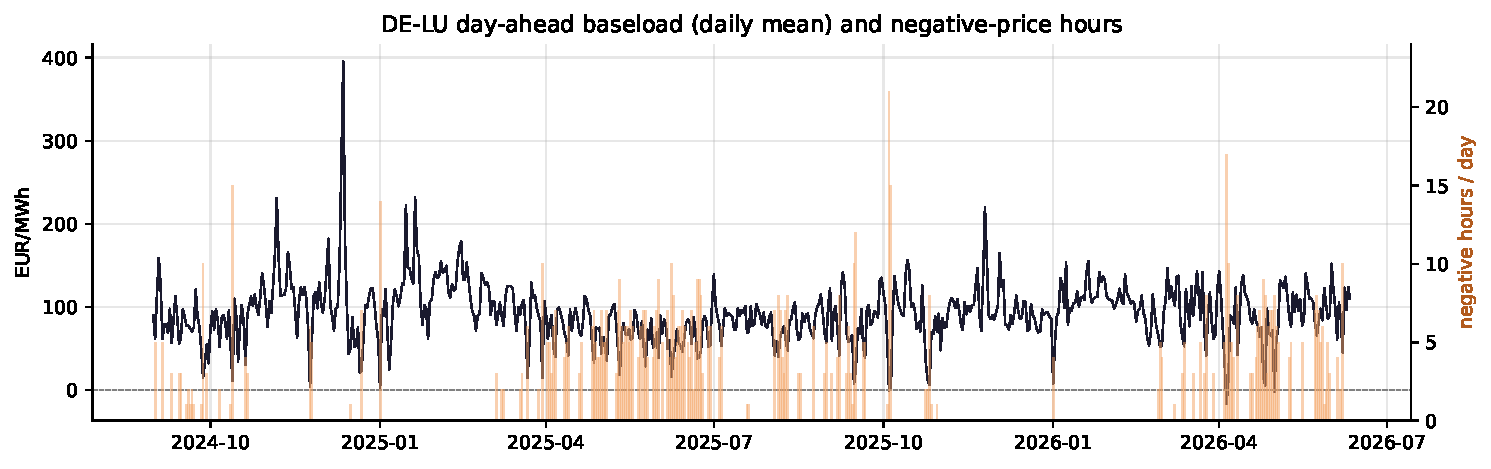
\includegraphics[width=0.94\textwidth]{01_price_history.pdf}
\caption{DE-LU day-ahead daily mean price and the number of negative-price
hours.  Hourly observations are retained for every model and metric.}
\label{fig:history}
\end{figure}

\section{Forecasting design}

\subsection{Features}

For target hour $t$ in delivery day $d$, the primary feature vector is
\[
  x_t = \bigl(
  y_{t-24},y_{t-48},y_{t-168},
  \overline y^{(d-1)}_t,s^{(d-1)}_t,\overline y^{(7d)}_t,
  S_t,W_t,R_t,\Delta_{24}R_t,C_t
  \bigr),
\]
where $S_t$ and $W_t$ are day-ahead solar and total-wind forecasts,
$R_t=S_t+W_t$, and $C_t$ contains hour, weekday, month, weekend, holiday, and
sine/cosine hour encodings.  The rolling price statistics are shifted by at
least 24 hours before aggregation.  Thus no realized price from delivery day
$d$ is used to forecast that day.

The day-over-day renewable change,
\[
  \Delta_{24}R_t = R_t-R_{t-24},
\]
provides a simple ramp indicator.  It is an input forecast difference, not a
realized generation change.  All continuous quantities are left in natural
units for the tree model.  Ridge is fitted inside a
standardization pipeline so its penalty does not depend on units.
The integer hour, weekday, and month fields are intentionally available to
LightGBM as ordered split variables; cyclic sine/cosine hour terms represent
the midnight boundary. This compact treatment avoids estimating sparse
categories in the short initial window, but it restricts calendar partitions
to contiguous integer groups and is therefore listed as model risk.

\subsection{Models}

The weekly naive forecast is
\[
  \widehat y^{\,N}_t=y_{t-168}.
\]
It preserves the same weekday-hour shape and is difficult to beat only when
the market changes little week to week.  Its weakness is deliberate: it
provides a transparent reference, not a straw-man claim that all persistence
models are equivalent.

Ridge estimates
\[
  \widehat\beta_\lambda
  =\arg\min_{\beta}\sum_{t\in\mathcal T}
    (y_t-\beta_0-x_t^\top\beta)^2+\lambda\|\beta\|_2^2,
  \qquad \lambda=10.
\]
The penalty is fixed before the reported out-of-sample window.  No
hyperparameter selection uses test losses.

The stronger linear benchmark fits the same standardized Ridge specification
separately for each of the 24 local delivery-hour labels. DST duplicate hours
share the same hour-specific model. This adds intraday coefficient flexibility
without using test outcomes or introducing a hyperparameter search. It is
LEAR-like in hourly structure, but it is not the full high-dimensional LEAR
benchmark of \cite{lago2021}.

LightGBM estimates an additive tree model
\[
  \widehat f_M(x)=\sum_{m=1}^{M}\nu h_m(x),
\]
with $M=600$, learning rate $\nu=0.05$, 63 leaves, minimum leaf sample size
40, row subsampling 0.9, column subsampling 0.9, and $\ell_2$ regularization
1.  The random seed is 42.  Deterministic column-wise training is requested
explicitly.  These values are frozen; the paper does not report a search over
alternative hyperparameters.

\subsection{Expanding-window protocol}

Let $D_1,\ldots,D_{365}$ be the final 365 local delivery days.  For each
$D_i$, the training set contains every feature row with local date strictly
less than $D_i$.  Models are re-estimated when $i\equiv1\pmod 7$ and reused
for the next six delivery days.  The entire day, including a DST transition,
is predicted as one test block.

The design is intentionally test-heavy: 365 local days are reserved for
evaluation, while the first forecast is trained on
\InitialTrainingDays{} complete feature days. The initial model has not seen
a full prior annual cycle. To expose possible cold-start effects, the paper
also reports LightGBM MAE after excluding the first 90 test days.

\begin{proposition}[No target leakage through the split]
If each primary feature for delivery day $d$ is measurable before the D-1
auction and the training mask is $\{t:\operatorname{day}(t)<d\}$, then no
realized price from day $d$ enters either the fitted parameters or the feature
vector used to forecast day $d$.
\end{proposition}

\begin{proof}
The training mask excludes every timestamp with local delivery date $d$.
Each rolling price feature is shifted by at least 24 hours, and the remaining
primary features are a deterministic calendar or a day-ahead TSO forecast.
Therefore both the fitted sample and $x_t$ for $t\in d$ are measurable before
the target prices $y_t$ are realized.
\end{proof}

This proposition is conditional on the source labels and the implementation.
It does not establish that an upstream archive never revised a historical
record.  That remaining data-vintage risk is discussed in
Section~\ref{sec:limitations}.

\subsection{Point metrics}

For errors $e_t=\widehat y_t-y_t$ over $n$ hours,
\[
  \MAE=\frac{1}{n}\sum_{t=1}^{n}|e_t|,
  \qquad
  \RMSE=\sqrt{\frac{1}{n}\sum_{t=1}^{n}e_t^2},
  \qquad
  \operatorname{Bias}=\frac{1}{n}\sum_{t=1}^{n}e_t.
\]
MAE is primary because it remains interpretable with negative prices and
does not square the already influential spikes.  RMSE and the 95th percentile
of absolute error retain information about tails.

For uncertainty in MAE, the code first computes a mean absolute error for each
local delivery day and resamples overlapping seven-day blocks of the 365 daily
values 4,000 times \cite{kunsch1989}. The 2.5 and 97.5 percentiles form the
reported interval. This preserves within-day dependence and short inter-day
dependence aligned with the HAC lag; it remains unable to reproduce arbitrary
long regime shifts.

\subsection{Loss-differential test}

For comparator $A$ and candidate $B$, define daily absolute loss
\[
  L_{d,m}=\frac{1}{H_d}\sum_{h=1}^{H_d}
  |y_{d,h}-\widehat y^{\,m}_{d,h}|,
  \qquad
  \delta_d=L_{d,A}-L_{d,B}.
\]
Positive $\delta_d$ favors $B$.  The sample mean $\bar\delta$ is divided by a
Newey--West standard error with Bartlett weights and lag seven:
\[
  \widehat\Omega
  =\widehat\gamma_0+
   2\sum_{k=1}^{7}\left(1-\frac{k}{8}\right)\widehat\gamma_k,
  \qquad
  t=\frac{\bar\delta}{\sqrt{\widehat\Omega/n_d}}.
\]
The statistic is multiplied by the Harvey--Leybourne--Newbold small-sample
factor for a one-day forecast horizon \cite{harvey1997}. This remains a
Diebold--Mariano-style comparison on daily $L_1$ loss. The weekly naive
forecast is also an input feature, so that comparison shares the nested-model
problem studied by \cite{clarkwest2007}; Clark--West's squared-error adjustment
does not transfer directly to the primary absolute-error loss. The fixed HAC
lag and reference distribution remain approximations, and $p$-values are
strength-of-evidence diagnostics rather than exact finite-sample tests.

\subsection{Prequential intervals}

Let $a_t=|y_t-\widehat y_t|$ be the absolute residual.  Before predicting
delivery day $d$, the interval procedure takes residuals from the previous
60 delivery days, provided at least 30 days exist.  With $n_c$ calibration
residuals and $\alpha=0.10$, it sets
\[
  q_d = Q_{\lceil(n_c+1)(1-\alpha)\rceil/n_c}
        \left(\{a_t:\operatorname{day}(t)<d\}\right),
\]
using the higher empirical quantile, and reports
\[
  C_{d,h}=[\widehat y_{d,h}-q_d,\widehat y_{d,h}+q_d].
\]
The coefficients of the point model are not refitted by the interval wrapper.
The construction is strictly prequential in residual time but pools all hours
into one radius.  Hour-specific coverage therefore remains an essential
diagnostic. Alongside coverage and width, the artifact reports the proper
central interval score and two endpoint pinball losses \cite{gneiting2007}.
Hour-by-hour two-sided binomial tests are reported both unadjusted and with
Holm multiplicity correction.

\subsection{Prompt-proxy translation}

The model's next-day baseload fair value is
\[
  F_d=\frac{1}{H_d}\sum_h\widehat y_{d,h}.
\]
Because licensed EEX front-week settlements are not distributed with the
artifact, the prompt proxy is the trailing $w$-day realized day-ahead
baseload,
\[
  P_{d,w}=\frac{1}{w}\sum_{j=1}^{w}\overline y_{d-j}.
\]
The gap $G_{d,w}=F_d-P_{d,w}$ is standardized using a trailing 60-day mean and
standard deviation.  A long direction is recorded when $z_{d,w}>\tau$, a
short direction when $z_{d,w}<-\tau$, and neutral otherwise.

For direction $s_d\in\{-1,0,1\}$, the descriptive outcome is
\[
  R_d=s_d\left(
  \frac{1}{7}\sum_{j=0}^{6}\overline y_{d+j}-P_{d,w}
  \right).
\]
The seven-day forward average creates overlapping outcomes.  A fourteen-day
moving-block bootstrap \cite{kunsch1989} is therefore used for the default
$(w,\tau)=(7,0.75)$
summary.  The final six days have no complete forward outcome and are
right-censored.  They remain available for a current view but are excluded
from performance statistics.

\section{Empirical results}

\subsection{Point accuracy}

Table~\ref{tab:models} reports the full-year comparison.  LightGBM reaches an
MAE of \PrimaryMAE{} EUR/MWh, against \HourlyRidgeMAE{} for hourly Ridge,
\RidgeMAE{} for pooled Ridge, and \NaiveMAE{} for the weekly naive forecast.
The primary model's RMSE is
\PrimaryRMSE{}, larger than MAE as expected in a spiky market, and its bias is
\PrimaryBias{} EUR/MWh.  The negative bias indicates systematic
underprediction on average, a warning that the model should not be judged on
MAE alone.

After excluding the first 90 test days, LightGBM MAE over the remaining
\PostWarmupDays{} days is \PostWarmupMAE{} EUR/MWh. This diagnostic separates
the short initial training history from the headline full-year score without
silently discarding a difficult part of the declared test.

A strictly prequential intercept correction is also reported as a sensitivity,
not substituted into the primary forecast. On the common post-calibration
window, the uncorrected MAE and bias are \BiasWindowMAE{} and
\BiasWindowBias{} EUR/MWh; subtracting the prior-60-day mean residual changes
them to \BiasCorrectedMAE{} and \BiasCorrectedBias{}. This quantifies the
available bias correction while avoiding an ex-post full-sample intercept.

\begin{table}[t]
\centering
\caption{One-year expanding-window point-forecast accuracy. MAE intervals use
4,000 seven-day moving-block bootstrap draws of delivery-day summaries.}
\label{tab:models}
\small
\resizebox{\textwidth}{!}{\begin{tabular}{lrrrrr}
\toprule
Model & MAE [95\% CI] & RMSE & Bias & Median AE & 95th pct. AE \\
\midrule
Weekly naive & 32.89 [29.23, 36.74] & 51.21 & -0.87 & 19.27 & 102.48 \\
Pooled Ridge & 17.11 [16.04, 18.26] & 25.41 & -3.23 & 13.24 & 42.18 \\
Hourly Ridge (24 models) & 15.73 [14.78, 16.75] & 23.48 & -3.32 & 12.22 & 39.19 \\
LightGBM & 13.59 [12.39, 14.86] & 22.22 & -3.72 & 9.09 & 38.61 \\
\bottomrule
\end{tabular}
}
\end{table}

\begin{figure}[t]
\centering
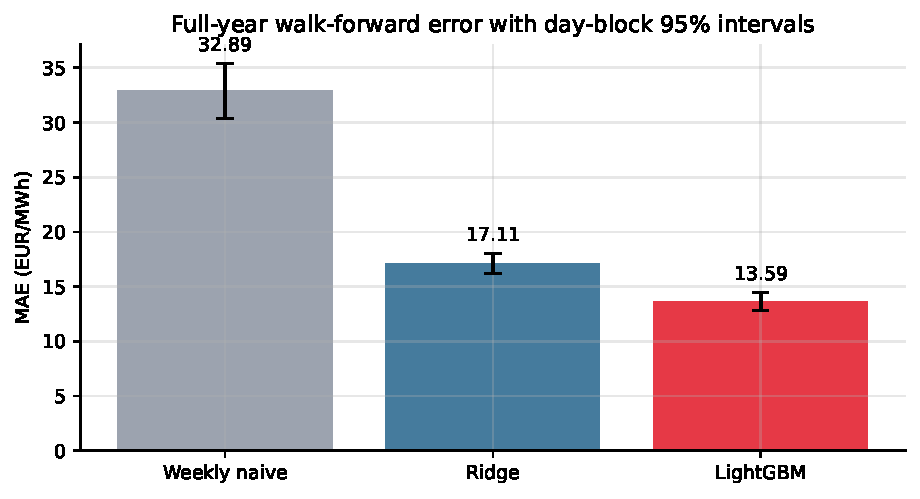
\includegraphics[width=0.92\textwidth]{07_model_uncertainty.pdf}
\caption{MAE and seven-day moving-block bootstrap 95\% intervals. Intervals
describe variability across this sample, not model or data-vintage risk.}
\label{fig:model-ci}
\end{figure}

Figure~\ref{fig:recent} illustrates the last fourteen delivery days.  The
nonlinear forecast tracks daily shape more closely than the weekly naive
profile, but misses several sharp ramps.  Figure~\ref{fig:scatter} gives the
full OOS scatter.  Compression toward the center is visible: high realized
prices are underpredicted and some low prices are overpredicted.

\begin{figure}[t]
\centering

\includegraphics[width=0.94\textwidth]{02_pred_vs_actual.pdf}
\caption{Hourly out-of-sample forecasts for the final fourteen days.}
\label{fig:recent}
\end{figure}

\begin{figure}[t]
\centering
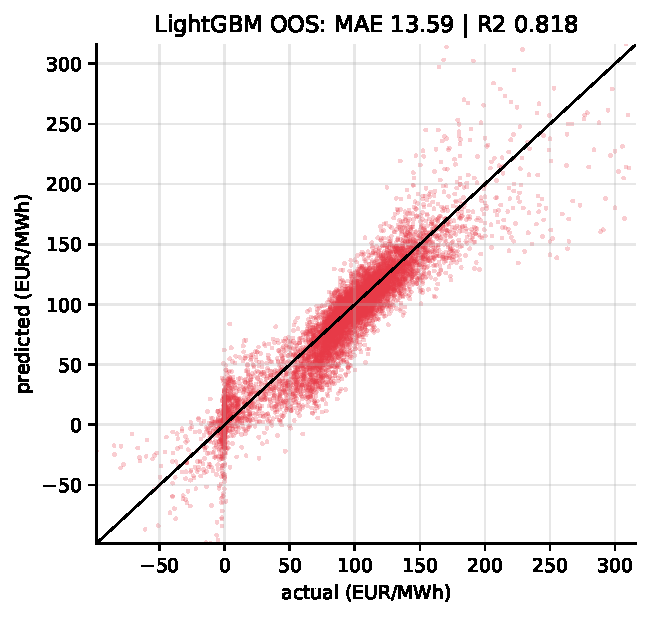
\includegraphics[width=0.68\textwidth]{03_scatter.pdf}
\caption{Observed versus LightGBM prices for all \OOSObservations{}
out-of-sample hours.}
\label{fig:scatter}
\end{figure}

\subsection{Statistical comparison and temporal stability}

The daily MAE gain is \DMGainNaive{} EUR/MWh relative to the naive model,
\DMGainRidge{} relative to pooled Ridge, and \DMGainHourlyRidge{} relative to
hourly Ridge. All HLN-corrected, autocorrelation-robust tests reject a zero mean
differential by a wide margin (Table~\ref{tab:dm}). These results support the
within-sample statement that the gain is persistent across days, rather than
being generated by one small group of hours.

\begin{table}[t]
\centering
\caption{Daily absolute-loss comparisons with seven-lag HAC standard errors
and the Harvey--Leybourne--Newbold finite-sample correction. Positive gains
favor LightGBM.}
\label{tab:dm}
\small
\begin{tabular}{lrrrr}
\toprule
Comparison & Mean daily MAE gain & HAC SE & Statistic & Two-sided $p$ \\
\midrule
LightGBM vs. Weekly naive & 19.29 & 1.64 & 11.80 & $2.05\times 10^{-27}$ \\
LightGBM vs. Ridge & 3.52 & 0.37 & 9.62 & $1.11\times 10^{-19}$ \\
\bottomrule
\end{tabular}

\end{table}

\begin{figure}[t]
\centering
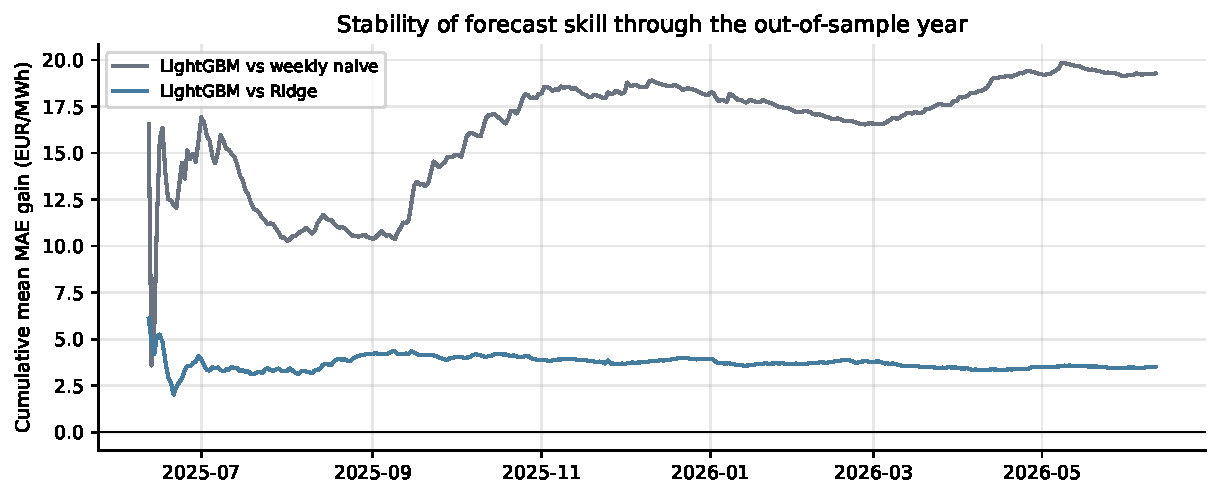
\includegraphics[width=0.90\textwidth]{08_cumulative_skill.pdf}
\caption{Expanding average daily MAE gain of LightGBM.  A line above zero
means that the comparator has incurred greater cumulative error.}
\label{fig:cumulative}
\end{figure}

Figure~\ref{fig:cumulative} shows that the expanding gain remains positive
throughout the year for both comparisons.  It should not be extrapolated
mechanically: the data include one recent annual cycle, not repeated crises,
fuel regimes, or structural policy changes.

\subsection{Hour, season, and feature importance}

Errors are not uniform through the day.  Figure~\ref{fig:hour} shows that
night and late-evening hours are easier, while daylight and the evening ramp
are harder. The nonlinear model's MAE is \MAENight{} EUR/MWh during hours
00--06, \MAEDaylight{} during hours 07--15,
\MAEEveningRamp{} during hours 16--21, and \MAELateEvening{} during hours
22--23. Spring has the largest seasonal MAE at \MAESpring{}, followed by
autumn at \MAEAutumn{}, summer at \MAESummer{}, and winter at
\MAEWinter{}.

\begin{figure}[t]
\centering

\includegraphics[width=0.84\textwidth]{04_mae_by_hour.pdf}
\caption{MAE by local delivery hour for all four models.}
\label{fig:hour}
\end{figure}

\begin{figure}[t]
\centering
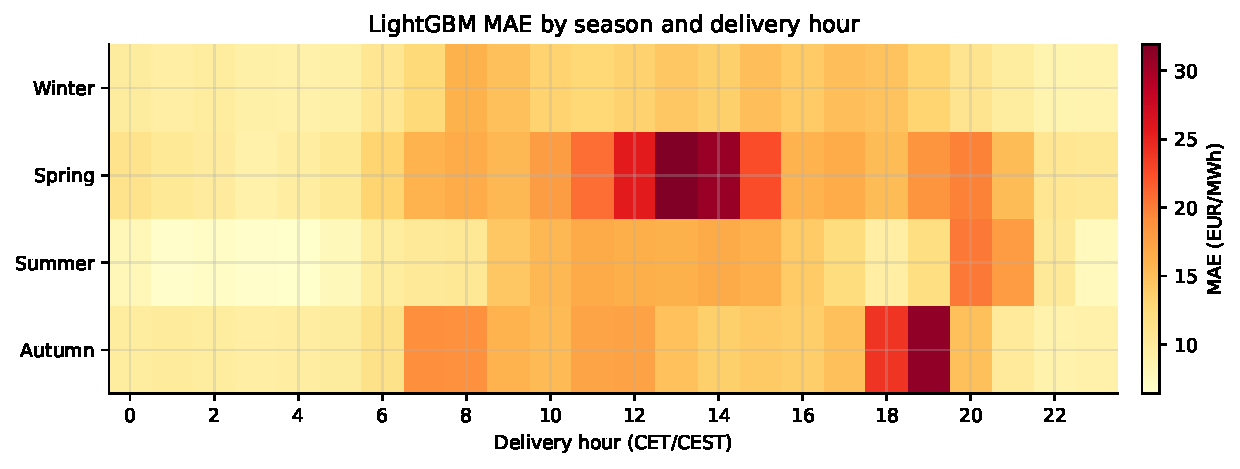
\includegraphics[width=0.94\textwidth]{09_season_hour_heatmap.pdf}
\caption{LightGBM MAE across season-hour cells.  The heat map makes clear
that aggregate calibration does not imply uniform conditional performance.}
\label{fig:season-hour}
\end{figure}

\begin{table}[t]
\centering
\caption{Primary-model errors by broad season and hour block.}
\label{tab:regimes}
\small
\begin{tabular}{llrrrr}
\toprule
Dimension & Regime & $n$ & MAE & RMSE & Bias \\
\midrule
Season & Autumn & 2,185 & 14.20 & 23.29 & -5.04 \\
Season & Spring & 2,207 & 16.30 & 28.08 & -6.02 \\
Season & Summer & 2,208 & 11.93 & 18.70 & -3.25 \\
Season & Winter & 2,160 & 11.92 & 17.03 & -0.50 \\
Hour Block & Daylight (07--15) & 3,285 & 16.65 & 27.29 & -4.38 \\
Hour Block & Evening ramp (16--21) & 2,190 & 15.49 & 24.74 & -4.24 \\
Hour Block & Late evening (22--23) & 730 & 9.16 & 12.73 & -2.40 \\
Hour Block & Night (00--06) & 2,555 & 9.30 & 12.80 & -2.78 \\
\bottomrule
\end{tabular}

\end{table}

Split-count importance is reported as an implementation diagnostic, not a
causal attribution.  The most frequently selected variables are the 24-hour
price lag, trailing weekly price mean, total renewable forecast, prior-day
price dispersion, prior-day mean, and day-over-day renewable change.
Correlated features can substitute for one another, so neither rank nor split
count measures economic marginal effect.

\begin{figure}[t]
\centering
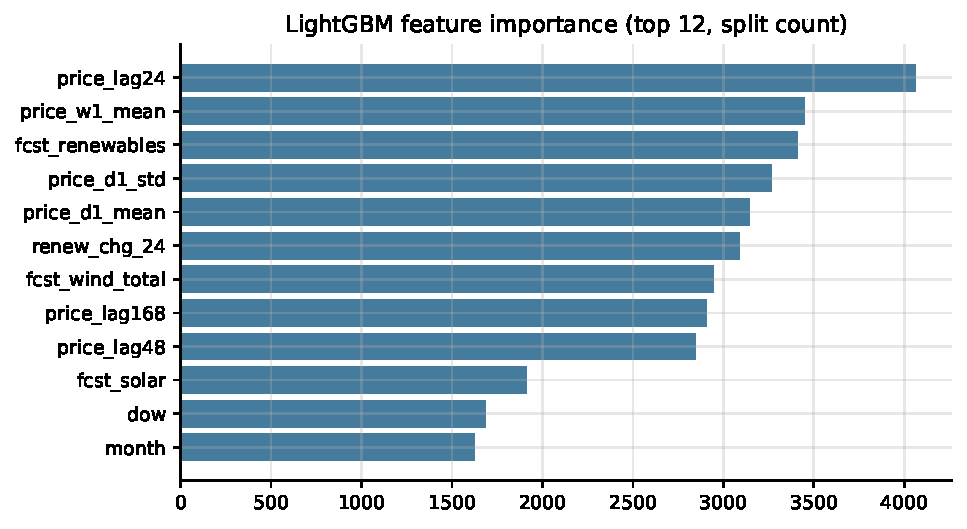
\includegraphics[width=0.76\textwidth]{05_feature_importance.pdf}
\caption{Average LightGBM split-count importance across the weekly refits.}
\label{fig:importance}
\end{figure}

\subsection{Ablation evidence}

Table~\ref{tab:ablation} and Figure~\ref{fig:ablation} keep the model class,
dates, refit cadence, and hyperparameters fixed while changing feature
families.  The weather-augmented sensitivity improves MAE by only
\WeatherDelta{} relative to the primary model.  This small difference is
inside the broad moving-block bootstrap intervals and does not justify relaxing the
information-vintage standard.

Renewables are materially more important.  Removing them leaves price history
and calendar variables and raises MAE by \NoRenewablesDelta{}.  A model with
renewables and calendar variables but no lagged prices obtains MAE
\FundamentalsCalendarMAE{}, which remains substantially better than
price-history plus calendar at \NoRenewablesMAE{}.
The result suggests complementarity: recent prices establish the prevailing
level while day-ahead renewable forecasts explain a large fraction of the
next-day deviation.

\begin{table}[t]
\centering
\caption{Feature-family ablations.  The weather-augmented row is a
sensitivity, not part of the primary ex-ante claim.}
\label{tab:ablation}
\small
\resizebox{\textwidth}{!}{\begin{tabular}{lrrrrr}
\toprule
Specification & Features & MAE & RMSE & Bias & MAE vs. primary \\
\midrule
Weather-augmented sensitivity & 22 & 13.49 & 21.85 & -3.59 & -0.8\% \\
Primary D-1 specification & 17 & 13.59 & 22.22 & -3.72 & +0.0\% \\
Renewables + calendar & 11 & 17.80 & 26.32 & -6.34 & +30.9\% \\
Price history + calendar & 13 & 25.14 & 37.14 & -0.84 & +84.9\% \\
Calendar only & 7 & 28.89 & 40.69 & +0.30 & +112.5\% \\
\bottomrule
\end{tabular}
}
\end{table}

\begin{figure}[t]
\centering
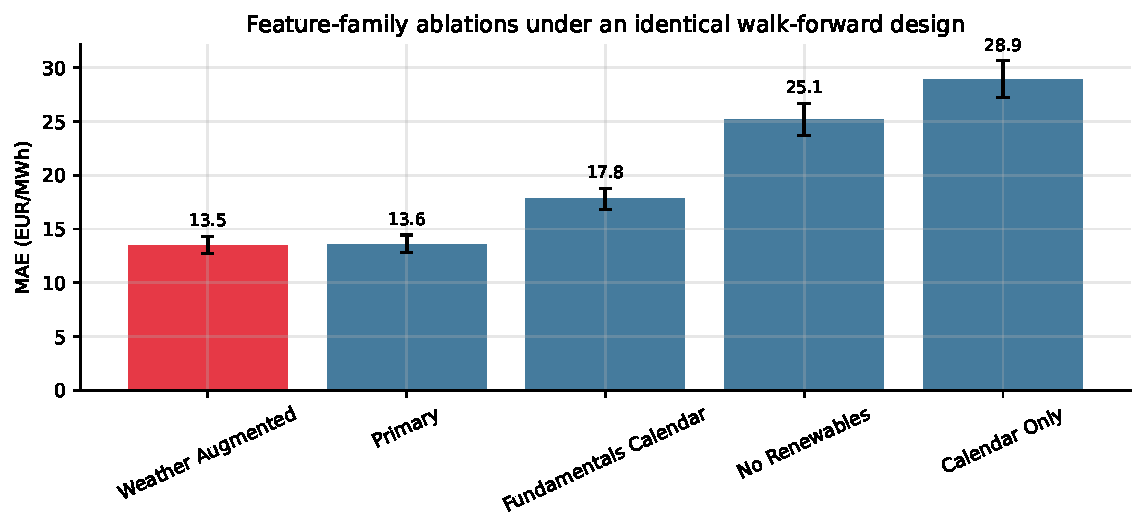
\includegraphics[width=0.88\textwidth]{12_ablation.pdf}
\caption{Ablation MAE with delivery-day bootstrap intervals.}
\label{fig:ablation}
\end{figure}

\subsection{Tail behavior}

Aggregate improvement coexists with economically relevant failure modes.
Table~\ref{tab:tails} divides the target into negative, regular, and
above-200 EUR/MWh hours. On regular hours, LightGBM obtains MAE
\RegularMAE{};
on negative hours, its MAE is \NegativeMAE{}; above 200, MAE
is \HighMAE{}.  The high-price bias is strongly negative, reflecting
regression toward the center.  The model predicts a value above 200 for only
\HighRecall{} of realized above-200 hours.

Ridge slightly outperforms LightGBM on negative-price hours in MAE, while
LightGBM is materially better in the high-price regime.  This is a useful
counterexample to any claim of uniform dominance.  A production forecaster
might combine models by regime, use a transformed target, add outages and
fuel-stack variables, or train an explicit tail objective. Variance-stabilizing
transformations designed for zero and negative electricity prices are a
particularly relevant extension for these documented tails
\cite{uniejewski2018}.

\begin{table}[t]
\centering
\caption{Errors conditional on realized price regime.  Conditioning on the
outcome is diagnostic and not an ex-ante trading rule.}
\label{tab:tails}
\small
\begin{tabular}{llrrr}
\toprule
Price regime (EUR/MWh) & Model & $n$ & MAE & Bias \\
\midrule
Price $<0$ & Weekly naive & 538 & 55.22 & +42.39 \\
Price $<0$ & Pooled Ridge & 538 & 21.47 & +0.99 \\
Price $<0$ & Hourly Ridge & 538 & 21.51 & -1.90 \\
Price $<0$ & LightGBM & 538 & 21.59 & +1.41 \\
$0\leq$ price $<200$ & Weekly naive & 8,065 & 29.74 & -1.60 \\
$0\leq$ price $<200$ & Pooled Ridge & 8,065 & 15.69 & -2.18 \\
$0\leq$ price $<200$ & Hourly Ridge & 8,065 & 14.34 & -2.22 \\
$0\leq$ price $<200$ & LightGBM & 8,065 & 12.14 & -3.33 \\
Price $\geq 200$ & Weekly naive & 157 & 118.34 & -111.46 \\
Price $\geq 200$ & Pooled Ridge & 157 & 74.99 & -71.42 \\
Price $\geq 200$ & Hourly Ridge & 157 & 67.07 & -64.58 \\
Price $\geq 200$ & LightGBM & 157 & 61.12 & -40.96 \\
\bottomrule
\end{tabular}

\end{table}

\begin{figure}[t]
\centering
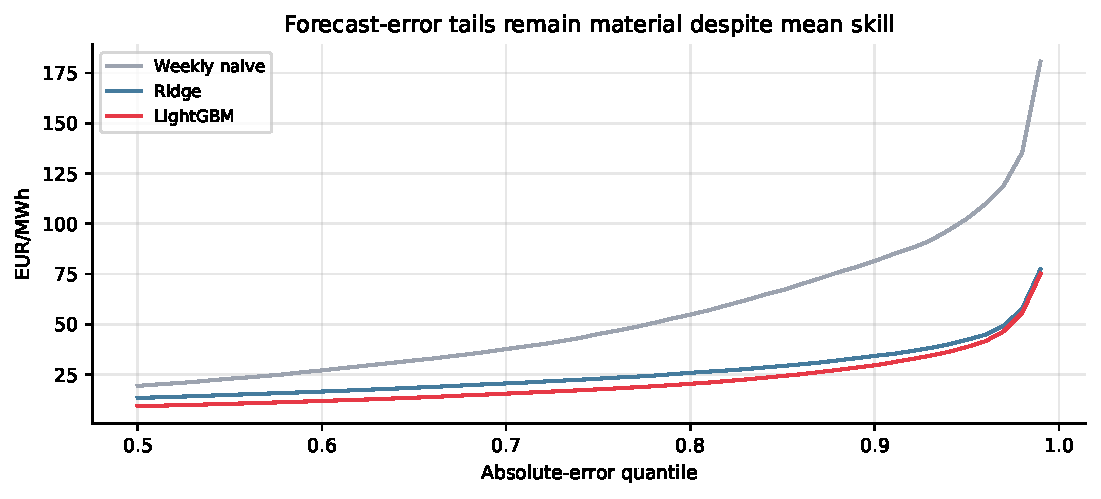
\includegraphics[width=0.80\textwidth]{14_error_quantiles.pdf}
\caption{Absolute-error quantile functions.  The nonlinear model's advantage
narrows in the far tail.}
\label{fig:error-quantiles}
\end{figure}

\subsection{Prequential interval performance}

Across \ConformalObservations{} evaluable hours after the minimum calibration period, the nominal
90\% interval covers \ConformalCoverage{} of outcomes with mean width
\ConformalWidth{} EUR/MWh and mean proper interval score
\ConformalIntervalScore{}. Aggregate calibration is close to the target.
Figure~\ref{fig:conformal-path} illustrates how the radius adapts through the
last fourteen days.

\begin{figure}[t]
\centering
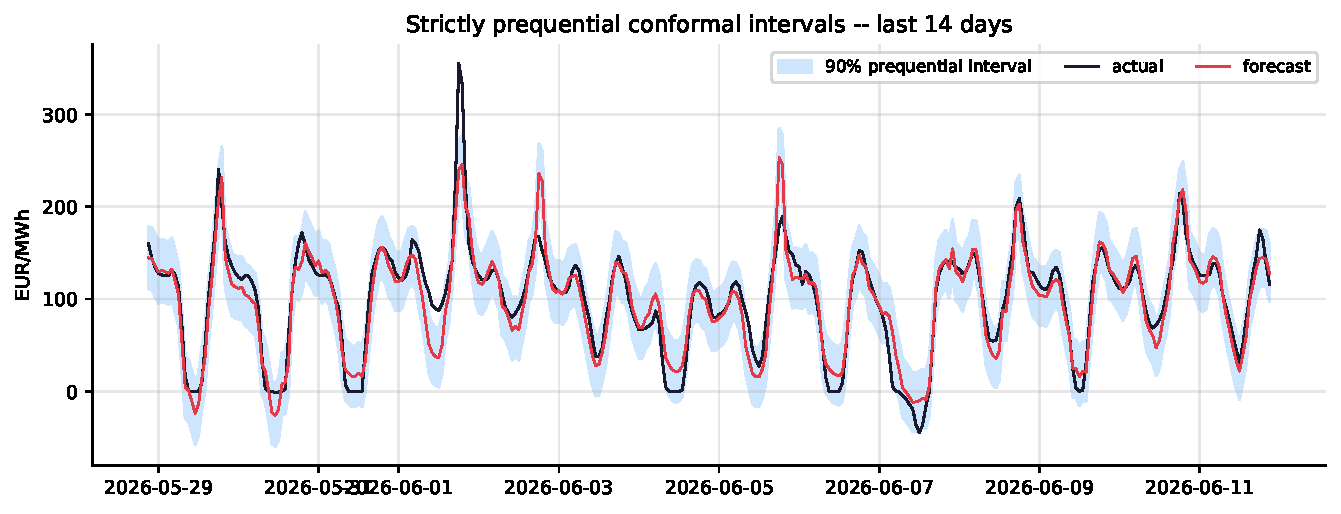
\includegraphics[width=0.94\textwidth]{10_conformal_path.pdf}
\caption{Forecasts and rolling-residual 90\% intervals over the final
fourteen days.}
\label{fig:conformal-path}
\end{figure}

The aggregate number conceals a formal conditional-coverage failure.
\ConditionalSignificantHours{} of the 24 hourly coverages differ from 90\%
under two-sided normal tests at 5\%:
\ConditionalUnderHours{} under-cover and \ConditionalOverHours{} over-cover.
After Holm correction across the 24 tests, \ConditionalHolmHours{} remain
significant. A common radius is too wide in easy hours and too narrow in
difficult hours. Hour-conditional residual pools, quantile regression, or an
adaptive conformal method \cite{gibbs2021} are natural extensions. Because the
time series is nonexchangeable, the marginal empirical rate remains a
descriptive validation result rather than a conditional or finite-sample
coverage theorem.

\begin{figure}[t]
\centering
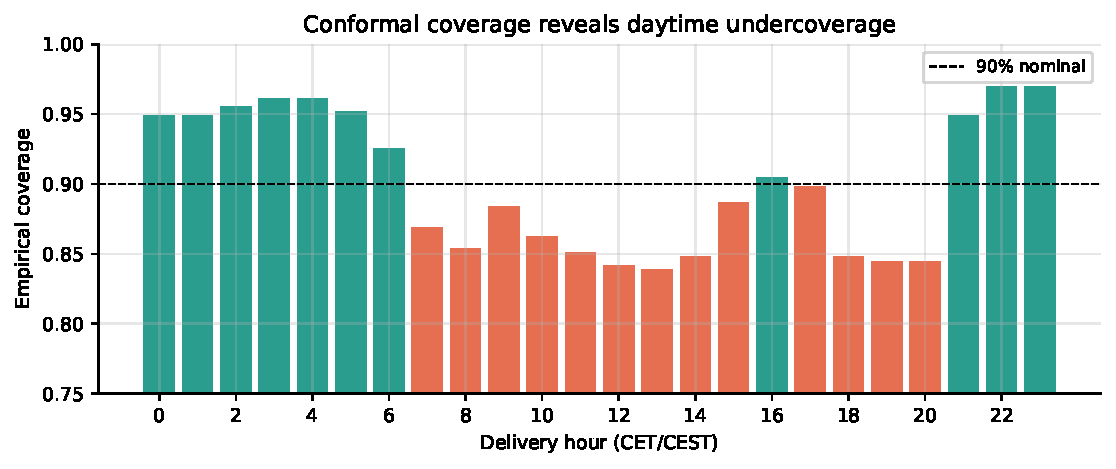
\includegraphics[width=0.84\textwidth]{11_conformal_coverage.pdf}
\caption{Empirical interval coverage by local delivery hour. Marginal
calibration masks widespread conditional rejection of the 90\% target.}
\label{fig:coverage-hour}
\end{figure}

\subsection{Prompt-proxy diagnostic}

Figure~\ref{fig:prompt} plots the next-day baseload fair value, the trailing
seven-day day-ahead prompt proxy, and the standardized gaps.  At the declared
$|z|>0.75$ threshold, \SignalActive{} active observations have complete
forward-week outcomes.  The directional hit rate is \SignalHit{} and the mean
signed spread is \SignalCaptured{} EUR/MWh.  A fourteen-day moving-block
bootstrap gives a hit-rate interval of
[\SignalHitLow{}, \SignalHitHigh{}] and a mean-spread interval of
[\SignalMeanLow{}, \SignalMeanHigh{}] EUR/MWh.

\begin{figure}[t]
\centering
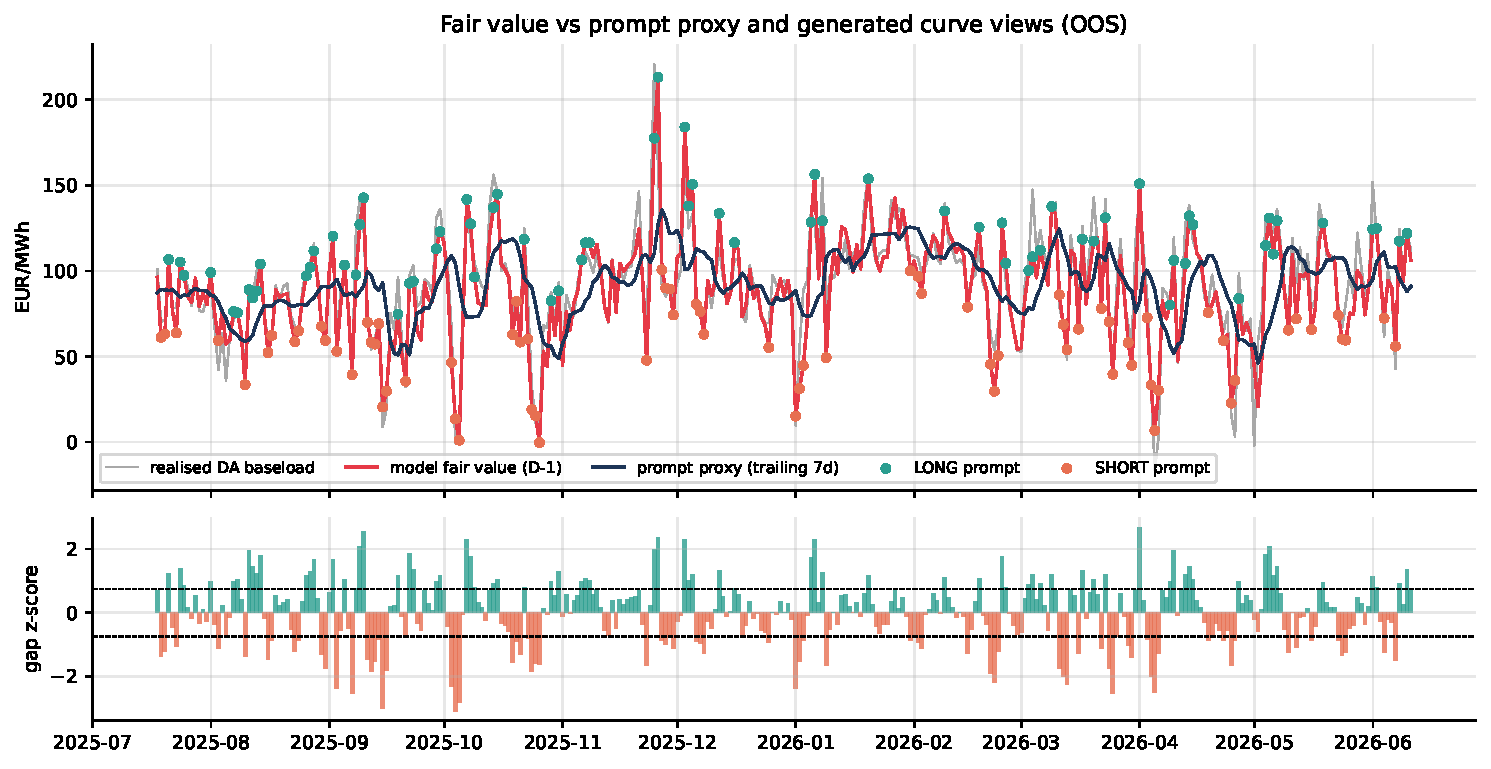
\includegraphics[width=0.94\textwidth]{06_fair_value_vs_prompt.pdf}
\caption{Next-day baseload fair value, trailing day-ahead prompt proxy, and
generated directions.  This is not an EEX forward backtest.}
\label{fig:prompt}
\end{figure}

Table~\ref{tab:signal-bounds} bounds the raw result. Always-long and weekly
naive references quantify simple persistence. Pooled and hourly Ridge show how
much of the direction survives a materially weaker point forecaster, while
perfect knowledge of day-D baseload is an infeasible upper bound for this
particular construction. LightGBM carries direction beyond weekly persistence,
but the proximity of the linear and perfect-information rows shows that much
of the headline hit rate is mechanical: day D enters the forward-week average
and the prompt spread is autocorrelated. This is evidence of directional
information, not model-specific alpha.

\begin{table}[t]
\centering
\caption{Bounds for the declared seven-day, $|z|>0.75$ prompt diagnostic.
Mean spread is signed EUR/MWh. ``Perfect day-D'' is deliberately infeasible.}
\label{tab:signal-bounds}
\small
\resizebox{\textwidth}{!}{\begin{tabular}{lcrrr}
\toprule
Signal input & Feasible & Active days & Hit rate & Mean spread \\
\midrule
Always long (no model signal) & yes & 352 & 48.3\% & 0.55 \\
Weekly naive fair value & yes & 121 & 54.5\% & 1.71 \\
Pooled Ridge fair value & yes & 148 & 71.6\% & 12.44 \\
Hourly Ridge fair value & yes & 150 & 73.3\% & 13.32 \\
LightGBM fair value & yes & 144 & 74.3\% & 13.25 \\
Perfect day-D baseload (infeasible) & no & 139 & 81.3\% & 14.96 \\
\bottomrule
\end{tabular}
}
\end{table}

Sensitivity matters. Raising the threshold generally increases the observed
hit rate and magnitude while sharply reducing the sample. The best-looking
ex-post cell is therefore not evidence for an optimized live threshold. The
value 0.75 is retained because it was declared in the prototype before this
expanded analysis.

\begin{table}[t]
\centering
\caption{Threshold sensitivity for the seven-day prompt proxy.  Mean and
median columns are signed forward-week spreads in EUR/MWh.}
\label{tab:signal}
\small
\begin{tabular}{rrrrrr}
\toprule
$|z|$ threshold & Active days & Hit rate & Mean spread & Median spread & Long/short \\
\midrule
0.50 & 200 & 71.5\% & 11.15 & 10.50 & 102/98 \\
0.75 & 144 & 74.3\% & 13.25 & 12.34 & 70/74 \\
1.00 & 105 & 79.0\% & 13.78 & 11.99 & 52/53 \\
1.25 & 72 & 83.3\% & 17.41 & 18.05 & 29/43 \\
1.50 & 47 & 80.9\% & 18.30 & 22.18 & 19/28 \\
2.00 & 21 & 76.2\% & 13.71 & 15.39 & 8/13 \\
\bottomrule
\end{tabular}

\end{table}

\begin{figure}[t]
\centering
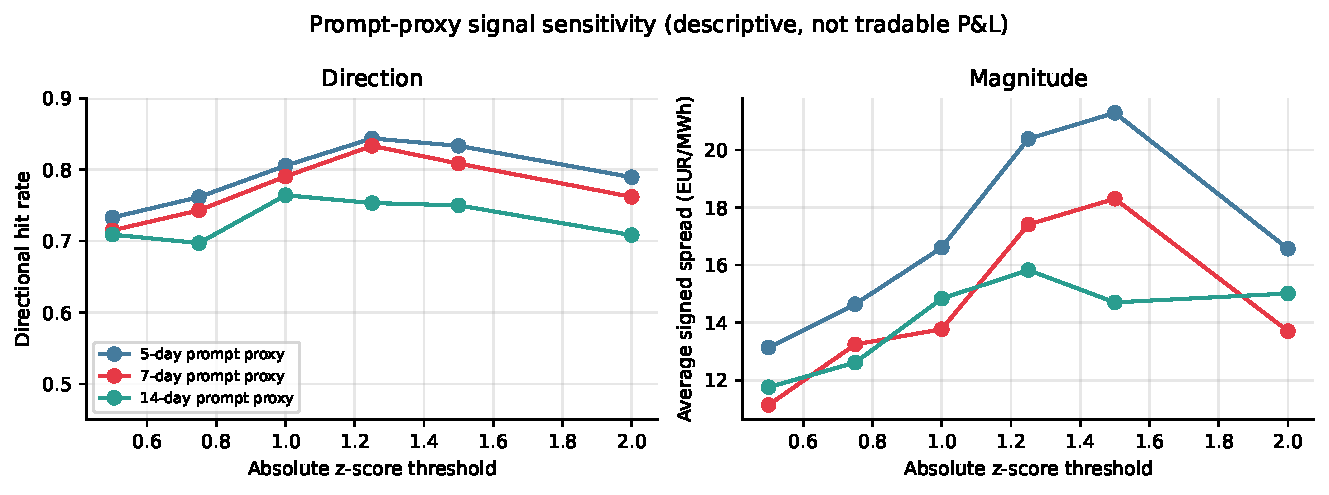
\includegraphics[width=0.92\textwidth]{13_signal_sensitivity.pdf}
\caption{Signal sensitivity across prompt windows and thresholds.  The
outcomes overlap and are descriptive only.}
\label{fig:signal-sensitivity}
\end{figure}

\section{Discussion}

\subsection{What the evidence supports}

The strongest conclusion is comparative and local.  Under one fixed
implementation, a complete OOS year, and the declared D-1 feature set,
LightGBM materially reduces absolute error relative to a weekly naive model
and both Ridge specifications. The improvement appears through the year,
survives daily dependence adjustments, and is not explained by the
ambiguous-vintage weather series. Renewable forecasts are a central source of
skill.

The artifact also shows why an MAE headline is insufficient.  The primary
model is negatively biased, its daytime interval coverage is weak, and its
error increases sharply in negative and high-price regimes.  Ridge is
competitive on negative prices.  These facts are not ancillary; they define
the operational boundary of the model. Likewise, the prompt diagnostic exceeds
weekly persistence but is largely shaped by its overlapping arithmetic rather
than unique LightGBM alpha.

\subsection{What the evidence does not support}

The results do not establish causal effects of renewable generation on
prices.  The feature importance and ablations measure predictive contribution
inside this design.  Renewables correlate with demand, outages, fuel costs,
and cross-border conditions that are not fully observed.

The results do not establish state-of-the-art performance.  The repository
does not compare with LEAR, neural networks, probabilistic gradient boosting,
or commercial forecast vendors.  It also does not tune LightGBM against the
test year.  This restraint makes the comparison easier to audit but narrower
than a comprehensive benchmark.

Finally, the prompt-proxy output is not a backtested financial return.
Licensed front-week settlements, bid-ask spreads, transaction costs, margin,
execution timing, and risk limits are absent.  A trailing day-ahead average
does not contain the forward risk premium.  The experiment measures whether a
standardized fair-value divergence aligns with subsequent day-ahead
baseload, nothing more.

\subsection{Operational interpretation}

A practical forecasting desk could use the point model as one component of a
larger process.  The next-day curve provides an hourly shape and a baseload
summary.  The prequential interval gives a first uncertainty band, while the
hourly coverage chart identifies where that band is least trustworthy.
Invalidation rules should include major TSO forecast revisions, REMIT
outages, fuel and carbon shocks, and an error beyond a rolling tolerance.

The current implementation deliberately keeps those rules outside the
statistical score.  Without timestamped outage, fuel, carbon, and actual
forward data, coding them into a historical strategy would create an illusion
of precision.

\section{Software artifact and reproducibility}

\subsection{Architecture}

The repository is divided into seven executable stages:

\begin{enumerate}[leftmargin=*,itemsep=2pt]
  \item \texttt{ingest.py} downloads and caches source responses;
  \item \texttt{qa.py} validates the assembled hourly dataset;
  \item \texttt{features.py} constructs the declared information set;
  \item \texttt{models.py} runs the full-year walk-forward experiment;
  \item \texttt{trading.py} builds the right-censoring-aware prompt proxy;
  \item \texttt{research.py} produces uncertainty, ablation, regime, and
  sensitivity evidence;
  \item \texttt{make\_figures.py} and
  \texttt{generate\_paper\_artifacts.py} render figures, tables, and macros
  directly from the frozen outputs.
\end{enumerate}

Tabular transformations use pandas \cite{mckinney2010}; standardized Ridge,
metrics, and preprocessing use scikit-learn \cite{pedregosa2011}. These
software dependencies are pinned in the paper environment.

The optional language-model component writes a short desk note from
pipeline-computed numbers.  It is excluded from every scientific result.  Its
dry-run mode logs the exact prompt without credentials or a network call.  No
paper table or figure depends on generated prose.

\subsection{Evidence lineage}

\begin{table}[H]
\centering
\caption{Lineage from numerical claim to executable evidence.}
\label{tab:lineage}
\small
\begin{tabular}{L{0.27\textwidth}L{0.26\textwidth}L{0.35\textwidth}}
\toprule
Claim & Producer & Frozen artifact \\
\midrule
Point accuracy and intervals & \texttt{models.py}, \texttt{research.py} &
\texttt{model\_comparison.csv}, \texttt{model\_daily\_losses.csv} \\
Loss-differential significance & \texttt{research.py} &
\texttt{dm\_tests.csv} \\
Feature-family contribution & \texttt{research.py} &
\texttt{ablation\_metrics.csv}, \texttt{ablation\_predictions.csv} \\
Regime and tail errors & \texttt{research.py} &
\texttt{regime\_metrics.csv}, \texttt{tail\_metrics.csv} \\
Prequential coverage & \texttt{research.py} &
\texttt{conformal\_diagnostics.csv},
\texttt{conformal\_hour\_tests.csv} \\
Bias sensitivity & \texttt{research.py} &
\texttt{bias\_correction\_diagnostics.csv} \\
Prompt-proxy sensitivity and bounds & \texttt{trading.py},
\texttt{research.py} &
\texttt{daily\_views.csv}, \texttt{signal\_sensitivity.csv},
\texttt{signal\_benchmarks.csv} \\
\bottomrule
\end{tabular}
\end{table}

Every figure is generated in both PNG and vector PDF form.  The README uses
PNGs; this paper uses the matching PDFs.  Generated LaTeX tables are not
manually transcribed.  Dataset and prediction hashes provide a quick audit
that a reported paper was built from the intended frozen state.

\subsection{Tests and deterministic controls}

The test suite checks price-lag direction, independent primary/weather sample
conditioning, QA invariants, the HLN/HAC sign convention, seeded moving-block
resampling, strictly prior conformal calibration, the exact 365-day OOS shape,
all four forecast columns, prompt right-censoring and benchmark bounds,
equality between primary ablation and frozen model predictions, conditional
coverage reconciliation, dataset hashing, and the presence of all fourteen
vector figures.

LightGBM uses an explicit seed and deterministic training mode.  Bootstrap
generators use fixed seeds.  Exact floating-point equality across operating
systems is not promised: compiler, math-library, and LightGBM versions can
change last-bit results.  The locked paper environment and committed CSV
evidence make such differences visible.

\section{Limitations and model risk}
\label{sec:limitations}

\begin{enumerate}[leftmargin=*,itemsep=5pt]
  \item \textbf{Sample length.}  The dataset spans roughly twenty-one months
  and the test covers one year.  Lago et al. \cite{lago2021} advocate longer
  multi-year evaluation.  This artifact does not cover multiple energy
  crises, policy regimes, or fuel cycles. More than half of the raw local days
  are reserved for testing, leaving only \InitialTrainingDays{} complete
  feature days before the first forecast and no full prior annual cycle.

  \item \textbf{Upstream revisions.}  The local code enforces chronological
  splits, but an upstream API may revise historical forecasts.  Raw response
  caching protects future reruns, not the first retrieval.  True vintage
  validation would require archive snapshots with issue timestamps.

  \item \textbf{Weather.}  The stitched Open-Meteo historical series is not a
  fixed D-1 forecast.  It is excluded from the primary claim.  The sensitivity
  must not be described as live-reproducible until fixed-lead runs are used.

  \item \textbf{Fundamental omissions.}  Load forecasts, outages,
  interconnector availability, hydro conditions, TTF gas, coal, EUA carbon,
  and neighboring-market forecasts are absent.  These omissions are likely
  material during scarcity and fuel-led moves.

  \item \textbf{Model selection.}  Hyperparameters are fixed rather than
  selected in a nested time-series validation.  That reduces researcher
  degrees of freedom but does not prove the chosen values are optimal.
  Calendar integers are treated as ordered tree-split variables; cyclic hour
  terms help, but noncontiguous weekday or month groupings are unavailable.

  \item \textbf{Intervals.} The symmetric pooled conformal radius assumes
  neither hour-specific scale nor asymmetric tails. Aggregate coverage near
  90\% coexists with formal hour-conditional rejection, and temporal
  dependence prevents a naive exchangeability guarantee.

  \item \textbf{Significance.} The HAC lag, seven-day moving-block bootstrap,
  HLN adjustment, and reference distribution are modeling choices. The naive
  forecast is nested in the feature set, while the primary loss is absolute
  rather than squared error. Extremely small $p$-values indicate strong sample
  evidence, not an immutable population ranking.

  \item \textbf{Prompt proxy.}  A trailing day-ahead mean is not a forward
  settlement and contains no explicit risk premium.  Overlapping forward-week
  outcomes, mechanical persistence, missing costs, and threshold exploration
  preclude a trading performance claim. Similar Ridge and LightGBM hit rates
  show that the raw success rate is not model-specific alpha.

  \item \textbf{Interpretability.}  Split-count importance is unstable under
  correlated features and is not causal.  Ablations are more informative but
  can also change interactions and model capacity.

  \item \textbf{Production readiness.}  The artifact has caching, QA, and
  deterministic outputs, but lacks a feature store, late-data policy,
  monitoring service-level objectives, access controls, and an audited
  execution interface.
\end{enumerate}

\section{Conclusion}

This paper presents a reproducible DE-LU day-ahead forecasting artifact that
treats information timing and uncertainty as first-class research objects.
On a complete out-of-sample year, the primary LightGBM model obtains
\PrimaryMAE{} EUR/MWh MAE and improves on a weekly naive model, pooled Ridge,
and the stronger hourly Ridge baseline. The gain is stable across the sample
and significant under an HLN-corrected daily autocorrelation-robust
comparison. Renewable forecasts account for a large share of predictive value.
The more permissive weather variant changes MAE only marginally and is
estimated on its own complete-case sample because its archive does not
preserve a fixed D-1 vintage.

The same evidence also limits the conclusion. Error remains large in negative
and above-200 price regimes; marginal 90\% interval coverage masks rejection
across many delivery hours; and the sample covers one recent year with a short
initial training history rather than multiple structural regimes. The
prompt-proxy experiment is bounded by persistence and perfect-information
references and is shown to be partly mechanical, not a forward-market
backtest.

The result is therefore best viewed as a publication-ready foundation:
source-backed, testable, and explicit about what remains unknown.  Extending
the data to multiple years, introducing fixed-vintage weather, load, outages,
fuel, carbon, and interconnector inputs, and evaluating conditional
probabilistic forecasts, variance-stabilized targets, and a full LEAR
implementation would turn that foundation into a broader empirical study.

\clearpage
\appendix

\section{Complete primary feature dictionary}

\begin{longtable}{p{0.25\textwidth}p{0.67\textwidth}}
\caption{Primary model features and their timing interpretation.}
\label{tab:features}\\
\toprule
Feature & Definition and timing \\
\midrule
\endfirsthead
\toprule
Feature & Definition and timing \\
\midrule
\endhead
\texttt{price\_lag24} & Same local-sequence hour one day earlier; auction
price already published before the current D-1 gate closure. \\
\texttt{price\_lag48} & Price two days earlier. \\
\texttt{price\_lag168} & Same hour one week earlier; also the naive forecast. \\
\texttt{price\_d1\_mean} & Mean of a 24-hour rolling window applied after a
24-hour shift. \\
\texttt{price\_d1\_std} & Standard deviation of the same shifted window. \\
\texttt{price\_w1\_mean} & Mean of the prior 168 hours after a 24-hour shift. \\
\texttt{fcst\_solar} & TSO day-ahead solar generation forecast in MW. \\
\texttt{fcst\_wind\_total} & Sum of onshore and offshore day-ahead wind
forecasts in MW. \\
\texttt{fcst\_renewables} & Solar plus total wind forecast. \\
\texttt{renew\_chg\_24} & Current day-ahead renewable forecast minus the
forecast at the same hourly position one day earlier. \\
\texttt{hour} & Europe/Berlin delivery hour. \\
\texttt{dow} & Local day of week. \\
\texttt{month} & Local calendar month. \\
\texttt{is\_weekend} & Indicator for Saturday or Sunday. \\
\texttt{is\_holiday} & German public-holiday indicator. \\
\texttt{hour\_sin}, \texttt{hour\_cos} & Cyclic encoding of local hour. \\
\bottomrule
\end{longtable}

\section{Executable algorithms}

\subsection{Algorithm A: walk-forward point forecasts}

\textbf{Input:} feature table, ordered local delivery days, 365-day test
window, seven-day refit cadence.

\begin{enumerate}[leftmargin=*]
  \item Select the final 365 distinct Europe/Berlin delivery days.
  \item For test day $D_i$, set the training mask to every row whose local day
  is strictly earlier than $D_i$.
  \item When $i$ is the first day of a seven-day block, fit standardized Ridge
  pooled across hours, 24 standardized hour-specific Ridge models, and
  deterministic LightGBM on the training mask.
  \item Predict every 23/24/25 target hour of $D_i$ with the same fitted
  models; copy the 168-hour lag as the naive prediction.
  \item Append timestamp, target, and all four predictions without shuffling.
  \item After the final day, compute metrics and save the exact prediction
  matrix to CSV.
\end{enumerate}

\textbf{Output:} \texttt{data/predictions\_oos.csv} and
\texttt{reports/model\_metrics.json}.

\subsection{Algorithm B: prequential interval}

\textbf{Input:} ordered point predictions and targets, nominal coverage
$1-\alpha=0.90$, 60-day residual window, 30-day minimum.

\begin{enumerate}[leftmargin=*]
  \item Group prediction timestamps by local delivery day.
  \item Before day $D_i$, collect absolute residuals only from days
  $D_{\max(1,i-60)},\ldots,D_{i-1}$.
  \item Compute the finite-sample-adjusted higher empirical quantile $q_i$.
  \item Apply the same symmetric radius to every hour of $D_i$.
  \item After observing the day, record coverage by timestamp and hour; only
  then can those residuals enter a later calibration window.
\end{enumerate}

\textbf{Output:} \texttt{data/conformal\_diagnostics.csv}.

\subsection{Algorithm C: feature-family ablation}

\begin{enumerate}[leftmargin=*]
  \item Freeze dates, targets, LightGBM parameters, seed, and refit cadence.
  \item Define the primary, weather-augmented, fundamentals-calendar,
  no-renewables, and calendar-only feature sets.
  \item Repeat the complete walk-forward procedure separately for each set.
  \item Reconcile the primary ablation predictions exactly with the frozen
  main-model column.
  \item Compute metrics and seven-day moving-block bootstrap intervals for
  every set.
\end{enumerate}

\textbf{Output:} \texttt{data/ablation\_predictions.csv} and
\texttt{data/ablation\_metrics.csv}.

\subsection{Algorithm D: prompt-proxy sensitivity}

\begin{enumerate}[leftmargin=*]
  \item Average hourly LightGBM predictions and targets into local daily
  baseload values.
  \item For prompt windows 5, 7, and 14, compute the trailing realized proxy
  and a 60-day rolling standardized fair-value gap.
  \item For thresholds 0.5 through 2.0, assign long, short, or neutral.
  \item Compute the realized D through D+6 baseload spread; mark the final six
  dates right-censored.
  \item For the declared 7-day, 0.75 configuration, resample fourteen-day
  moving blocks 4,000 times.
\end{enumerate}

\textbf{Output:} \texttt{data/daily\_views.csv} and
\texttt{data/signal\_sensitivity.csv}.

\section{Additional numerical tables}

\subsection{Regime results}

Table~\ref{tab:regimes} in the main paper reports season and hour blocks.
The complete machine-readable table additionally includes renewable
quartiles and all four models. For the primary model, MAE is
\RenewableQOneMAE{}, \RenewableQTwoMAE{}, \RenewableQThreeMAE{}, and
\RenewableQFourMAE{} EUR/MWh across increasing renewable quartiles. The
high-renewable quartile is the most difficult, consistent with greater risk
of saturation and negative-price conditions.

\subsection{Threshold grid}

The six rows in Table~\ref{tab:signal} should be read jointly.  Higher
thresholds select more extreme gaps and fewer dates.  Because the same sample
is used to display all cells, selecting the largest ex-post hit rate would
introduce multiple-comparison bias.  No row other than the predeclared 0.75
threshold is used for an uncertainty claim.

\section{Validation matrix and reproduction}

\begin{table}[h]
\centering
\caption{Validation matrix for the released artifact.}
\label{tab:validation}
\small
\begin{tabular}{p{0.28\textwidth}p{0.31\textwidth}p{0.30\textwidth}}
\toprule
Component & Property & Acceptance criterion \\
\midrule
Dataset grid & Complete UTC hours & Zero missing and duplicate timestamps \\
DST mapping & Local day length & Every full day has 23, 24, or 25 hours \\
Feature timing & Price lags & Exact 24/48/168-hour backward mapping \\
Walk-forward split & Test horizon & 365 local days, 8,760 rows \\
Linear benchmark & Hour-specific fit & 24 Ridge models, refit every seven days \\
Primary ablation & Evidence reconciliation & Exact equality with main
LightGBM predictions \\
Primary sample & Optional weather & Primary row inclusion independent of weather \\
Conformal order & Prequentiality & Future target perturbation cannot change
earlier radii \\
Conditional coverage & Hour tests & Raw and Holm-adjusted counts reconcile \\
Trading evaluation & Right-censoring & Incomplete D through D+6 outcomes
excluded \\
Paper figures & Vector outputs & One nonempty PDF for each of 14 figures \\
Evidence identity & Frozen data & SHA-256 matches the research report \\
\bottomrule
\end{tabular}
\end{table}

The shortest reproduction from the committed dataset is:

\begin{verbatim}
python -m pip install -r requirements-paper.txt
python src/qa.py
python src/models.py
python src/trading.py
python src/research.py
python src/make_figures.py
python scripts/generate_paper_artifacts.py
python -m pytest -q
bash scripts/build_paper.sh
\end{verbatim}

The first ingestion run is deliberately separate because it calls external
services and may observe revised upstream values.  To rebuild from source
APIs, run \texttt{python src/ingest.py} before the commands above, archive the
raw responses, and expect the dataset fingerprint to change.

\bibliographystyle{plain}
\bibliography{references}

\end{document}
